\documentclass[10pt]{beamer}

% Pacotes Extras
\usepackage{rotating}
\usepackage{dsfont}
\usepackage{comment}
\usepackage{xcolor}
\usepackage{xcolor-material}
\usepackage{xcolor-solarized}
\usepackage[cachedir=.mintedcache]{minted}
\usemintedstyle{material}
\usepackage{multicol}
\usepackage{listings}
\usepackage{ulem}
\usepackage{cancel}
\usepackage{lipsum} 
\usepackage{graphicx}
\usepackage{pstricks}
\usepackage{pst-plot}
\usepackage{pst-3dplot}
\usepackage{booktabs}
\usepackage{wrapfig}
\usepackage{chngcntr}
\counterwithin*{footnote}{section}
\usepackage{metalogo}
\usepackage{enumitem}
%\usepackage{caption}
%\usepackage{subcaption}
\usepackage{subfig}
\usepackage[most]{tcolorbox}
\tcbuselibrary{breakable}
\tcbuselibrary{minted}
\usetikzlibrary{decorations.pathmorphing} 
\tcbuselibrary{skins}
\usepackage{setspace}
\PassOptionsToPackage{hyphens}{url}\usepackage{hyperref}
\usepackage{xspace}
\usepackage{lscape}
\usepackage{pdfpages}

% Macros extras
\definecolor{preto}{HTML}{515151}

% Caixas das Dicas (pacote tcolorbox)
% Material Colors
%\newtcolorbox{marker}[1][]{enhanced,
%  before skip=10mm,after skip=10mm,
%  boxrule=0.4pt,left=5mm,right=2mm,top=1mm,bottom=1mm,
%  colback=MaterialAmberA100,
%  colupper=preto,
%  colframe=MaterialGrey900,
%  sharp corners,rounded corners=southeast,arc is angular,arc=3mm,
%  underlay={%
%    \path[fill=tcbcol@back!80!black] ([yshift=3mm]interior.south east)--++(-0.4,-0.1)--++(0.1,-0.2);
%    \path[draw=tcbcol@frame,shorten <=-0.05mm,shorten >=-0.05mm] ([yshift=3mm]interior.south east)--++(-0.4,-0.1)--++(0.1,-0.2);
%    \path[fill=MaterialYellow100!50!black,draw=none] (interior.south west) rectangle node[white]{\Huge\bfseries !} ([xshift=4mm]interior.north west);
%    },
%  drop fuzzy shadow,#1}
\newtcolorbox{marker}[1][]{enhanced,
  before skip=10mm,after skip=10mm,
  boxrule=1.4pt,left=6mm,right=3mm,top=2mm,bottom=2mm,
  colback=MaterialAmberA100!75,
  colupper=black,
  colframe=preto,
  underlay={%
    \path[fill=none] (frame.south west) rectangle node[preto]{\huge\bfseries !} ([xshift=7mm]frame.north west);
    }}
  
% Caixas dos Exemplos (pacote tcolorbox)
% Material Colors
\tcbset{
    texexp/.style={
        colframe=MaterialBlue900,
        colback=white,
        coltitle=white,
        fonttitle=\small\sffamily\bfseries,
        fontupper=\small, 
        fontlower=\small},
        example/.style 2 args={texexp,
        title={Exemplo \thetcbcounter: #1},label={#2}},
    }
    \newtcblisting{texexp}[1]{texexp,#1}
    \newtcblisting[auto counter,number within=section]{texexptitled}[3][]{%
        example={#2}{#3},#1}
    \newtcolorbox[use counter from=texexptitled]{texexptitledspec}[3][]{%
        example={#2}{#3},#1}

%\newtcolorbox[auto counter,number within=section,list inside=exam]{texercise}[4][]{%
%    texercisestyle,
%    listing file={respostas/texercise\thetcbcounter.tex},
%    label={exe:#2},
%    record={\string\processsol{respostas/texercise\thetcbcounter.tex}{#2}},
%    title={Exercício \thetcbcounter\hfill\mdseries Resposta na página \pageref{sol:#2}},
%    list text={\vspace{-1em}\hspace{1mm} #3 (Resposta na página \pageref{sol:#2}}), #1)}

% Caixas dos Exercícios e Soluções (pacote tcolorbox)  
% Material Colors
\NewTColorBox[auto counter,number within=chapter]{exercise}{m+O{}}{%
    enhanced,
    colframe=MaterialGreen900,
    colback=white,
    coltitle=white,
    fonttitle=\bfseries,
    underlay={\begin{tcbclipinterior}
        \shade[inner MaterialGreen900,outer color=white]
            (interior.north west) circle (2cm);
        \draw[help lines,step=5mm,MaterialGreen900,shift={(interior.north west)}]
            (interior.south west) grid (interior.north east);
        \end{tcbclipinterior}},
    title={Exercício~ \thetcbcounter:},
    label={exercise:#1},
    attach title to upper=\quad,
    after upper={\par\hfill\textcolor{white}%
        {\itshape Resposta na página~\pageref{solution:#1}}},
    lowerbox=ignored,
    savelowerto=docs/respostas/exercise-\thetcbcounter.tex,
    record={\string\solution{#1}{docs/respostas/exercise-\thetcbcounter.tex}},
    #2
}

% Esta é a lista de exercícios
\newtcolorbox[auto counter,number within=section,list inside=exam]{texercise}[4][]{%
    texercisestyle,
    listing file={docs/respostas/texercise\thetcbcounter.tex},
    label={exe:#2},
    record={\string\processsol{docs/respostas/texercise\thetcbcounter.tex}{#2}},
    title={Exercício \thetcbcounter\hfill\mdseries Resposta na página \pageref{sol:#2}},
    list text={\vspace{-1em}\hspace{1mm} #3 - resposta na página \pageref{sol:#2}}, #1)}
    
\tcbset{texercisestyle/.style={arc=0.5mm, colframe=MaterialGreen900,
    colback=white, coltitle=white,
    fonttitle=\small\sffamily\bfseries, fontupper=\small, fontlower=\small,
    listing options={style=tcblatex,texcsstyle=*\color{MaterialRed900}},
}}

% \usepackage{hyperref} % for phantomlabel
\newtcbinputlisting{\processsol}[2]{%
    texercisestyle,
    listing only,
    listing file={#1},
    phantomlabel={sol:#2},%
    title={Resposta do Exercício \ref{exe:#2} na página \pageref{exe:#2}},
}

% Caixa dos Comandos (pacote tcolorbox)
% Material Colors
\newtcblisting{commandshell}{colback=MaterialBlueGrey900,colupper=MaterialBlueGrey50,colframe=MaterialBlueGrey900!75!MaterialBlueGrey900,listing only,listing options={style=tcblatex,language=sh},
    every listing line={\textcolor{MaterialRed500}{\small\ttfamily\bfseries \$ }}}

%\newtcblisting{meucomando}{listing engine=minted,
%	minted style=colorful,
%	minted language=bash,
%	minted options={fontsize=\small,breaklines,autogobble,linenos,numbersep=3mm},
%	colback=MaterialAmber50,colframe=MaterialBlueGrey900,listing only,
%	left=5mm,enhanced,
%	overlay={\begin{tcbclipinterior}\fill[MaterialAmber600] (frame.south west)
%			rectangle ([xshift=5mm]frame.north west);\end{tcbclipinterior}}}

\newtcblisting{meucomando}{listing engine=minted,
	minted style=colorful,
	minted language=bash,
	minted options={fontsize=\small,breaklines,autogobble,linenos,numbersep=3mm},
	colback=blue!5!white,colupper=black,colframe=preto,listing only,
	left=5mm,enhanced,
	overlay={\begin{tcbclipinterior}\fill[red!20!blue!20!white] (frame.south west)
			rectangle ([xshift=5mm]frame.north west);\end{tcbclipinterior}}}

% Sentenças individuais Loren Lipsum (pacote lipsum)
% REF: https://tex.stackexchange.com/questions/254901/one-sentence-of-dummy-text
% store a big set of sentences
\unpacklipsum[1-100] % it was \UnpackLipsum before version 2.0
\ExplSyntaxOn
% unpack \lipsumexp
\seq_new:N \g_lipsum_sentences_seq
\cs_generate_variant:Nn \seq_set_split:Nnn { NnV }
\seq_gset_split:NnV \g_lipsum_sentences_seq {.~} \lipsumexp

\NewDocumentCommand{\lipsumsentence}{>{\SplitArgument{1}{-}}O{1-7}}
 {
  \lipsumsentenceaux #1
 }
\NewDocumentCommand{\lipsumsentenceaux}{mm}
 {
  \IfNoValueTF { #2 }
   {
    \seq_item:Nn \g_lipsum_sentences_seq { #1 }.~
   }
   {
    \int_step_inline:nnnn { #1 } { 1 } { #2 }
     {
      \seq_item:Nn \g_lipsum_sentences_seq { ##1 }.~
     }
   }
 }
\ExplSyntaxOff


\usetheme{metropolis}

\usefonttheme[onlymath]{serif}
\usefonttheme{professionalfonts}
\usepackage{mathspec} 
\metroset{titleformat=allsmallcaps} % smallcaps

\setbeamercolor{alerted text}{fg=InpeLaranja}
\setbeamercolor{frametitle}{bg=InpeAzul}
\setbeamercolor{normal text}{fg=black}
\setbeamercolor{progress bar}{bg=InpeLaranja,fg=InpeAzul}
\setbeamercolor{title separator}{bg=InpeLaranja,fg=InpeLaranja}
\setbeamercolor{background canvas}{bg=white}

\setbeamertemplate{caption}[numbered]

\AtBeginSubsection[
  {\frame<beamer>{\frametitle{Sumário}   
    \tableofcontents[currentsection,currentsubsection]}}%
]%
{
  \frame<beamer>{ 
    \frametitle{Sumário}
    \begin{multicols}{2}
    \tableofcontents[currentsection,currentsubsection]
    \end{multicols}
    }
}

\title{Introdução ao \LaTeX}
\subtitle{Partes I e II}
\date{02 e 03 de Março de 2020}
\author{Carlos Frederico Bastarz (CPTEC/INPE)}
\institute{Instituto Nacional de Pesquisas Espaciais (INPE)}
\titlegraphic{\hfill
\includegraphics[height=1.5cm]{figs/layout/inpe_logo.png}}

\makeatletter
\patchcmd{\beamer@sectionintoc}{\vskip1.5em}{\vskip0.75em}{}{}
\makeatother

\begin{document}
\maketitle

\begin{frame}[c]{Sumário}
    \vspace{2em}
    \begin{multicols}{2}
        \begin{minipage}{0.49\textwidth}
           \vspace{12mm}
           \setbeamertemplate{section in toc}[sections numbered]
           \tableofcontents[hideallsubsections]
        \end{minipage}
        \begin{minipage}{0.49\textwidth}
            
\includegraphics[width=\textwidth]{./figs/ctan_lion_350x350.pdf}
        \end{minipage}
    \end{multicols}
\end{frame}

\section{Introdução}

\begin{frame}{O \LaTeX{}}
	\begin{block}{Por que utilizar o \LaTeX{}?}
		\begin{itemize}
			\pause
			\item Com o \LaTeX{} se produz documentos bonitos e bem estruturados;
			\pause
			\item Pode-se utilizar estilos pré-definidos ou customizados;
			\pause
			\item Você foca no conteúdo;
			\pause
			\item Você é desafiado.
		\end{itemize}
	\end{block}
\end{frame}

\begin{frame}{O \LaTeX{}}
	\begin{block}{É difícil aprender o \LaTeX{}?}
		\begin{itemize}
			\item \onslide<2-> Não é difícil, mas há uma curva de aprendizado;
			\item \onslide<3-> O \LaTeX{} parece uma linguagem de marcação;
			\item \onslide<4-> Ele permite a criação de \textit{macros}\footnotemark[1]
			\item \onslide<5-> Você é desafiado.
			\only<4->\footnotetext[1]{\textit{Macros} podem ser muito simples ou complexas. A propósito, esta é uma nota de rodapé!}
		\end{itemize}
	\end{block}
\end{frame}

\begin{frame}{O \LaTeX{}}
	\begin{block}{Que tipo de coisas bonitas pode-se fazer com o \LaTeX{}?}
		\begin{itemize}
			\item \onslide<2-> Esta apresentação {\large\Cooley}\footnotemark[1]
			\item \onslide<3-> Equações;
			\item \onslide<4-> Tabelas;
			\item \onslide<5-> Figuras em alta resolução (PDF!);
			\item \onslide<6-> Sua tese, dissertação, artigo, relatório, pôster, livro, etc;
			\item \onslide<7-> Qualquer tipo de documento que se queira produzir.
			\only<2->\footnotetext[1]{Este \textit{emoji} foi inserido utilizando-se o pacote {\tt tikzsymbols}. Esta apresentação é feita utilizando-se a classe {\tt beamer}.}
		\end{itemize}
	\end{block}
\end{frame}

\begin{frame}{O \LaTeX{}}
	\begin{block}{Qual é o aspecto das equações\footnote{Neste \textit{slide}, são utilizados três ambientes diferentes: {\tt equation*}, {\tt align} e {\tt gather}.} no \LaTeX{}?}
	    \vspace{-1em}
		\begin{center}
		        \begin{equation*}
		            \oint_C (Ldx + Mdy) = \iint_D \bigg(\frac{\partial{M}}{\partial{x}} - \frac{\partial{L}}{\partial{y}}\bigg)dxdy
		        \end{equation*}
			\vspace{-1em}
			\begin{align}
 				x            & = 1 + 2y + 3z \\ 
				3x -  y + 2z & = 0           \\
				2x +  y      & = 2 - z             
			\end{align}
			\vspace{-1em}		
			\begin{gather}
				x            = 1 + 2y + 3z \\ 
				3x -  y + 2z = 0           \\
				2x +  y      = 2 - z
			\end{gather}	
		\end{center}		
	\end{block}
\end{frame}

\begin{frame}[fragile]{O \LaTeX{}}
	\begin{block}{Tabelas no \LaTeX{}?}
		\begin{table}
			\scriptsize
			\caption{Uma tabela\footnote{Para produzir esta tabela utilizou-se o ambiente {\tt table} e os pacotes {\tt tabularx}, {\tt booktabs} e {\tt lipsum}.} com células mescladas.}
			\begin{tabularx}{\textwidth}{X X X X}
				\toprule
				\multicolumn{4}{c}{\textbf{4 Células Mescladas (colunas)}} \\
				\midrule
				\multicolumn{2}{c}{\textbf{2 Células Mescladas (colunas)}} & \multicolumn{2}{c}{\textbf{2 Células Mescladas (colunas)}} \\
				\midrule
				\multicolumn{1}{c}{\textbf{Coluna 1}} & \multicolumn{1}{c}{\textbf{Coluna 2}} & 
				\multicolumn{1}{c}{\textbf{Coluna 3}} & \multicolumn{1}{c}{\textbf{Coluna 4}} \\
				\midrule
				\lipsumsentence[1-2] & \lipsumsentence[3-4] & \lipsumsentence[5-6] & \lipsumsentence[7-8] \\
				\bottomrule
			\end{tabularx}
		\end{table}
	\end{block}
\end{frame}

\begin{frame}{O \LaTeX{}}
	\begin{block}{E as figuras\footnote{{\scriptsize Este diagrama foi incorporado a partir de um arquivo PDF com o ambiente {\tt figure} e o comando {\tt includegraphics}.}} no \LaTeX{}?}
    \vspace{-0.5em}
		\begin{figure}
				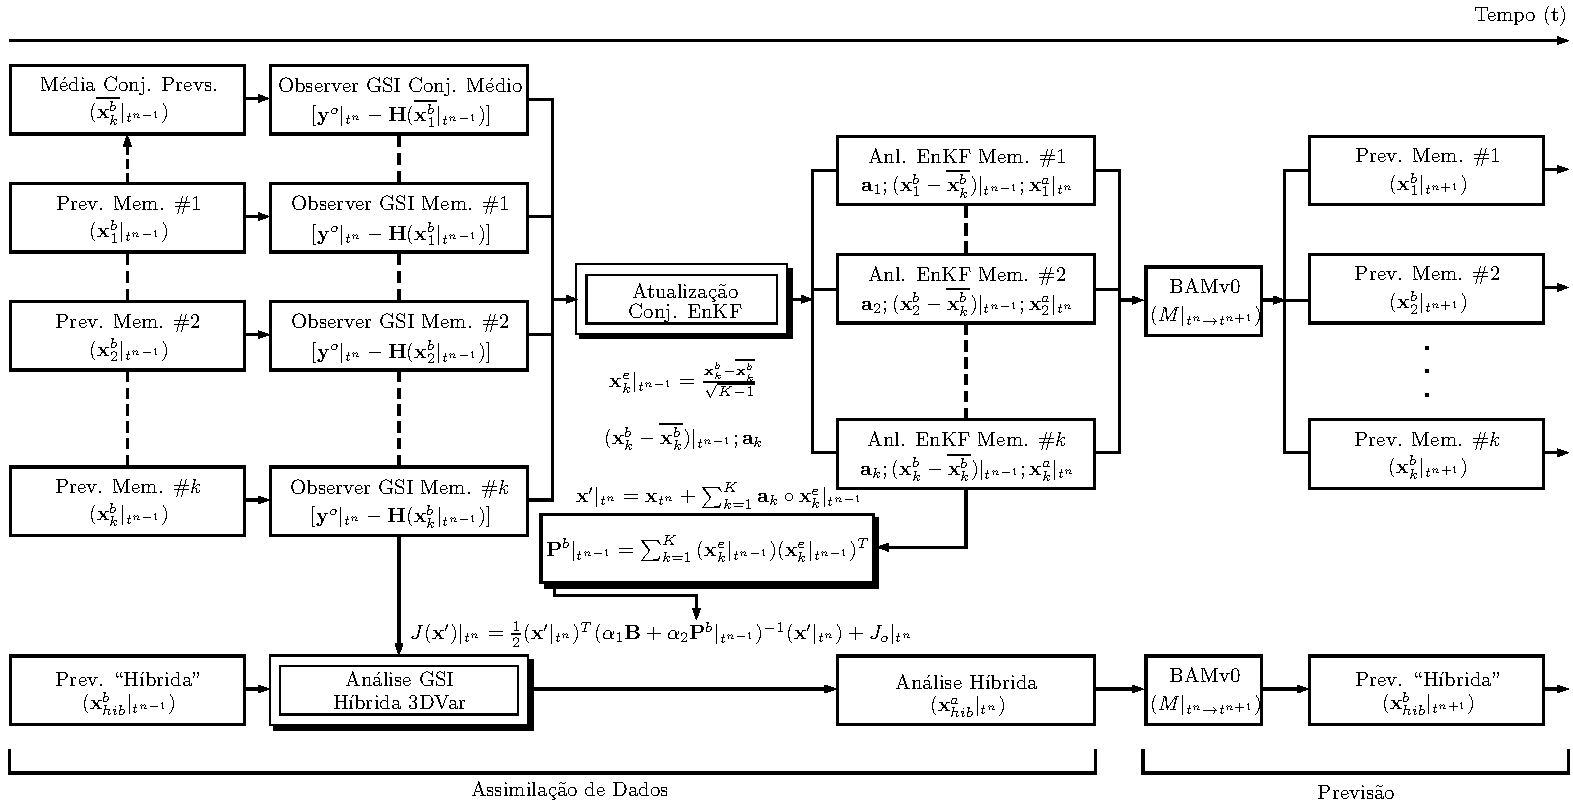
\includegraphics[scale=0.5]{./figs/diagrama_hibrido_novo_pt-tempos.pdf}
				\caption{Exemplo de um diagrama produzido no programa \LaTeX\textit{Draw}.}
		\end{figure}
	\end{block}
\end{frame}

\section{Parte I - Preparação}

\subsection{Escolhendo e Instalando o Compilador}

\begin{frame}{Como fazer tudo isso funcionar?}
O \LaTeX{} é uma linguagem de marcação que é interpretada por um \textbf{compilador} que se encarrega de mostrar o resultado em um arquivo final.
    \pause
	\begin{block}{Compiladores}
		\begin{itemize}
			\item Linux: \TeX{}\textit{Live}
			\item \textit{Microsoft Windows}: \TeX{}\textit{Live}
			\item Mac OS: Mac\TeX{}
		\end{itemize}
	\end{block}
\end{frame}

\begin{frame}[fragile]{Linux}
\begin{block}{Linux}
\vspace{0.5em}
No Linux, o \LaTeX{} pode ser facilmente instalado.
\begin{meucomandot}{Debian e derivados}
sudo apt install texlive-full
\end{meucomandot}
ou
\begin{meucomandot}{Red Hat e derivados}
sudo dnf install texlive-scheme-full
\end{meucomandot}
\end{block}
\end{frame}

\begin{frame}[fragile]{\textit{Microsoft Windows} e MacOS}
\begin{block}{\textit{Microsoft Windows}}
\vspace{0.5em}
No \textit{Microsoft Windows}, basta baixar e instalar o pacote \url{http://mirror.ctan.org/systems/texlive/tlnet/install-tl-windows.exe}
\end{block}

\begin{block}{Mac OS}
\vspace{0.5em}
No Mac OS, basta baixar e instalar o pacote \url{http://tug.org/cgi-bin/mactex-download/MacTeX.pkg} 
Pode-se também instalar pela linha de comando:
\begin{meucomandot}{Mac OS}
brew install caskroom/cask/brew-cask
brew cask install mactex
\end{meucomandot}
\end{block}
\end{frame}

\section{Parte II - Entendendo o \LaTeX{}}

\begingroup
\setbeamercolor{background canvas}{bg=InpeLaranja!90}
\begin{frame}[plain,fragile]{}
\begin{texexptitled}[center, enhanced jigsaw, width=0.99\paperwidth, height=0.99\paperheight, middle=2mm, listing side comment, righthand width=5cm, compilable listing, run latex, run dvips, run ps2pdf, pdf comment, comment style={raster columns=1},freeze pdf]{Um documento \LaTeX{} mínimo}{exe_doc}
\documentclass[10pt]{article}
% Este é o preâmbulo
\usepackage[utf8]{inputenc}
\usepackage{lipsum}

\title{Título}
\author{Nome}
\date{\today}

% A partir daqui inicia-se o documento
\begin{document}
\maketitle

\section{Seção}

\lipsum[1-3]
\end{document}
\end{texexptitled}
\end{frame}
\endgroup

\begin{frame}{Compilação de um documento \LaTeX{}}
\tikzstyle{format} = [draw, thin, fill=blue!20]
\tikzstyle{medium} = [ellipse, draw, thin, fill=green!20, minimum height=2.5em]
\begin{figure}
\vspace{5em}
\begin{tikzpicture}[node distance=3cm, auto,>=latex', thick]
    % We need to set at bounding box first. Otherwise the diagram
    % will change position for each frame.
    \path[use as bounding box] (-1,0) rectangle (10,-2);
    \path[->]<1-> node[format] (tex) {arq. {\tt .tex}};
    \path[->]<2-> node[format, right of=tex] (dvi) {arq. {\tt .dvi}}
                  (tex) edge node {\LaTeX} (dvi);
    \path[->]<3-> node[format, right of=dvi] (ps) {arq. {\tt .ps}}
                  node[medium, below of=dvi] (screen) {visualização}
                  (dvi) edge node {dvips} (ps)
                        edge node[swap] {xdvi} (screen);
    \path[->]<4-> node[format, right of=ps] (pdf) {arq. {\tt .pdf}}
                  node[medium, below of=ps] (print) {impressão}
                  (ps) edge node {ps2pdf} (pdf)
                       edge node[swap] {gs} (screen)
                       edge (print);
    \path[->]<5-> (pdf) edge (screen)
                        edge (print);
    \path[->, draw]<6-> (tex) -- +(0,1) -| node[near start] {pdf\LaTeX} (pdf);
\end{tikzpicture}
\vspace{2.5em}
\visible<6>{\caption{Etapas envolvidas na compilação de um documento \LaTeX{}. Adaptado de \url{http://www.texample.net/tikz/examples/tex-workflow/}.}}
\end{figure}
\end{frame}

\begin{frame}{Compilação de um documento \LaTeX{}}
\vspace{1em}
\begin{table}
\caption{Alguns tipos de compiladores \LaTeX{}.}
\vspace{-0.5em}
\begin{center}
    \begin{tabular}{p{2cm}p{8cm}}
    \toprule
    \textbf{Seção} & \textbf{Comando} \\
    \midrule
    \LaTeX{}    & Compilador \LaTeX{} puro, gera saída DVI, necessita do pacote {\tt inputenc} \\
    pdf\LaTeX{} & Compilador \LaTeX{} puro, gera saída em PDF, necessita do pacote {\tt inputenc} \\
    \XeLaTeX{}  & Compilador \LaTeX{} avançado, gera saída em PDF, não necessita do pacote {\tt inputenc}, suporta \textit{OpenType} \\
    Lua\LaTeX{} & Compilador \LaTeX{} avançado, gera saída em PDF, não necessita do pacote {\tt inputenc}, permite uso da linguagem Lua, suporta \textit{OpenType} \\
    \bottomrule
    \end{tabular}
\end{center}
\end{table}
\end{frame}

\begin{frame}{Compilação de um documento \LaTeX{}}
A forma como a compilação é feita vai depender de:
\begin{itemize}
    \item Editor;
    \item Sistema operacional.
\end{itemize}
Na linha de comando (eg., Linux, MacOS ou \textit{Microsoft Windows}\footnote{Considerando-se que o \textit{Windows Subsystem for Linux} e o \LaTeX{} estão instalados.}) a compilação segue da seguinte forma:
\end{frame}

\begin{frame}[fragile]{Compilação de um documento \LaTeX{}}
    \begin{block}{Linha de comando\footnote{Se for utilizado o compilador \XeLaTeX{}, o arquivo PDF será criado automaticamente. Além disso, estes comandos aceitam opções.}}
        \vspace{0.5em}
        \begin{meucomandot}{Documento simples}
            latex documento.tex
            dvips documento.dvi
            ps2pdf documento.ps
        \end{meucomandot}
    
        \begin{meucomandot}{Documento com referência Bib\TeX{}}
            latex documento.tex
            bibtex documento
            latex documento
            latex documento
        \end{meucomandot}
    \end{block}
\end{frame}

\begin{frame}{Compilação de um documento \LaTeX{}}
    \begin{block}{Exercício}
        \vspace{0.5em}
        Abra um editor de textos no seu computador e digite um documento mínimo com a classe {\tt article} e fonte de {\tt 10pt}. Utilize o pacote {\tt lipsum} para gerar alguns parágrafos de texto. Compile o documento com o {\tt latex}, {\tt pdflatex} e {\tt xelatex} e gere a saída em PDF. 
        Experimente também:
        \begingroup
        %\def{\labelenumi}{\arabic{enumi}.}
        %https://tex.stackexchange.com/questions/3455/problem-with-enumerate-package-in-beamer-class
        %\def\labelenumi{\theenumi}
        \begin{enumerate}
            \item Insira um sumário ao documento com o comando \mintinline{latex}{\tableofcontents};
            \item Altere a classe do documento para {\tt book}, {\tt report} e {\tt letter}.
        \end{enumerate}
        \endgroup
    \end{block}
\end{frame}

\begin{frame}{Compilação de um documento \LaTeX{}}
    \vspace{1.5em}
    \begin{block}{Editor local \TeX\textit{Studio}}
      \vspace{-3em}
	    \begin{figure}
		    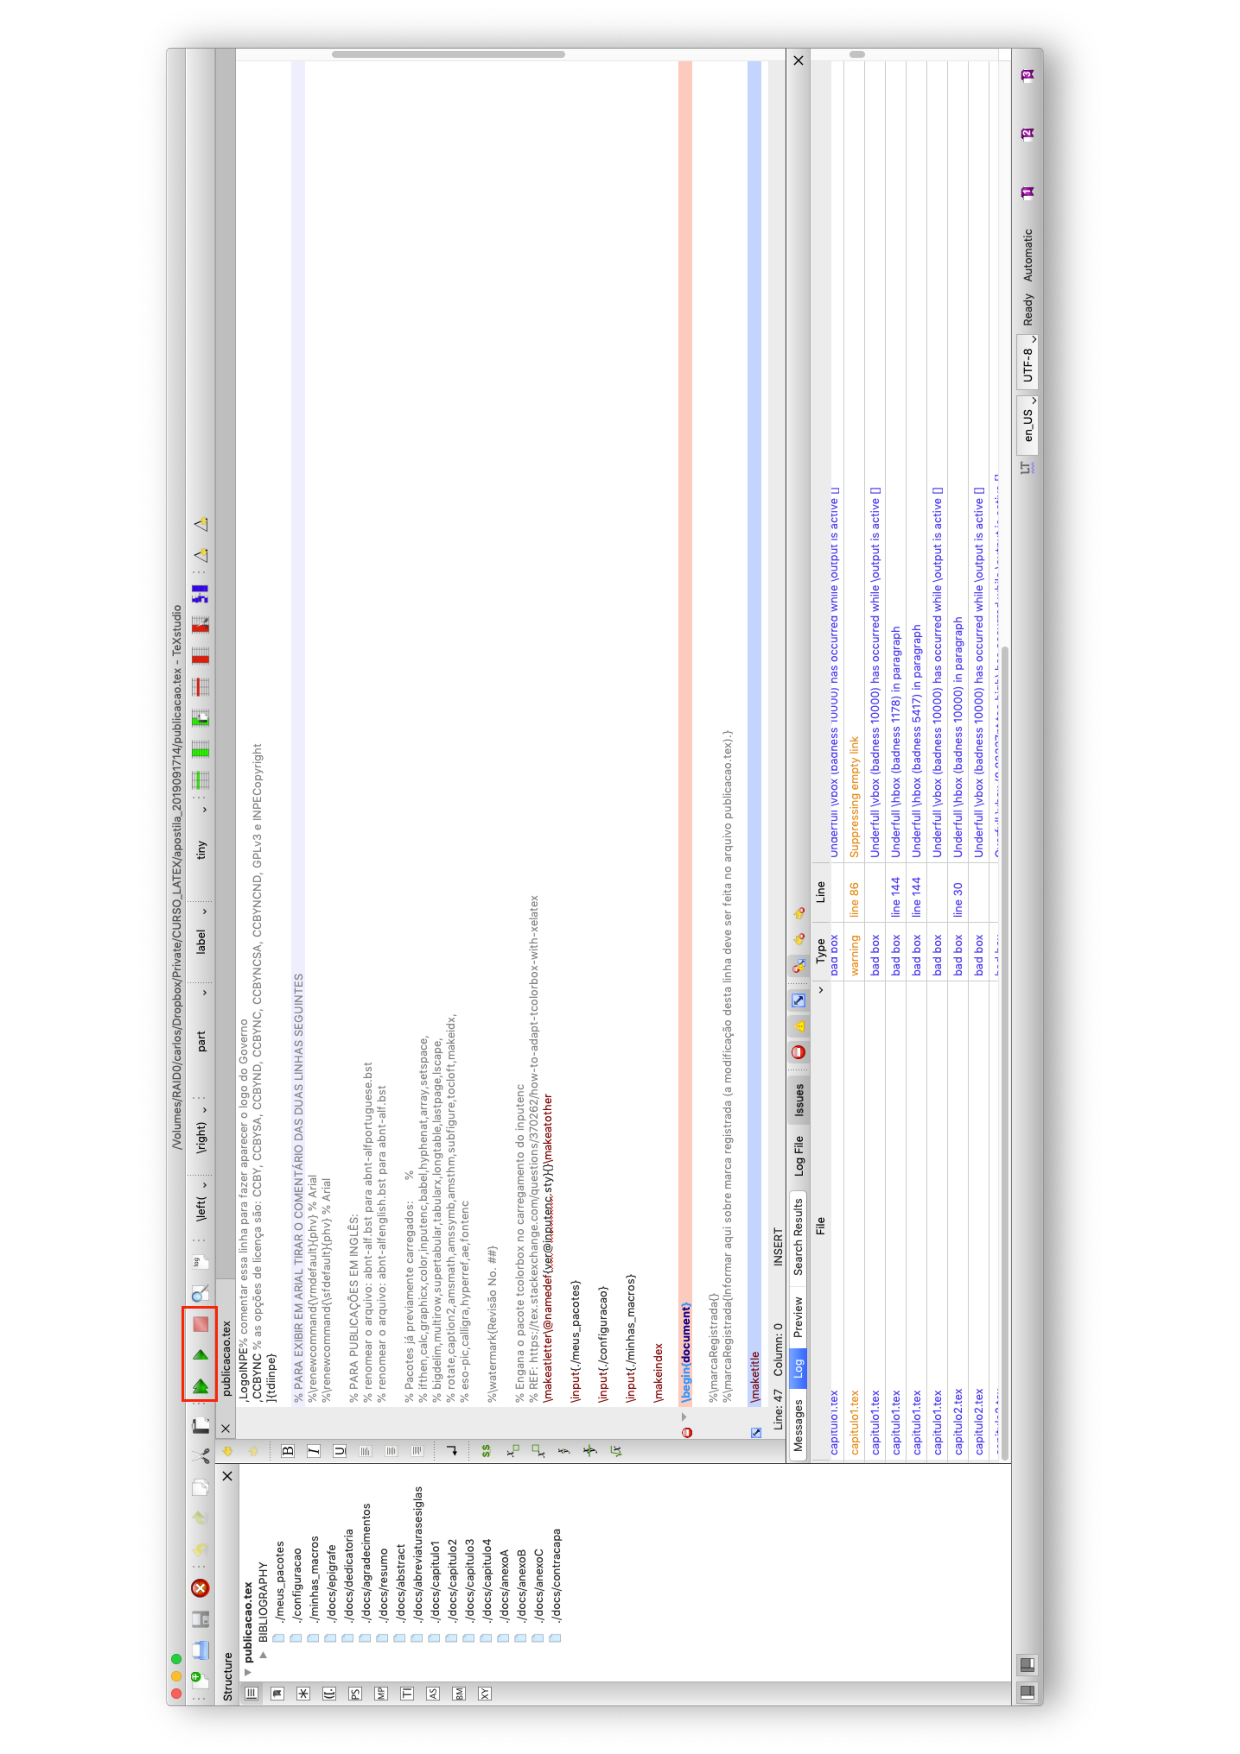
\includegraphics[width=0.65\textwidth,angle=-90]{./figs/texstudio.pdf}
		    \vspace{-2.5em}
		    \caption{Compilação de um documento \LaTeX{} no \TeX\textit{Studio} com o compilador \XeLaTeX{}.}
	    \end{figure}
    \end{block}
\end{frame}

\begin{frame}{Compilação de um documento \LaTeX{}}
    \vspace{1.5em}
    \begin{block}{Editor \textit{online} Overleaf}
      \vspace{-3em}
	    \begin{figure}
		    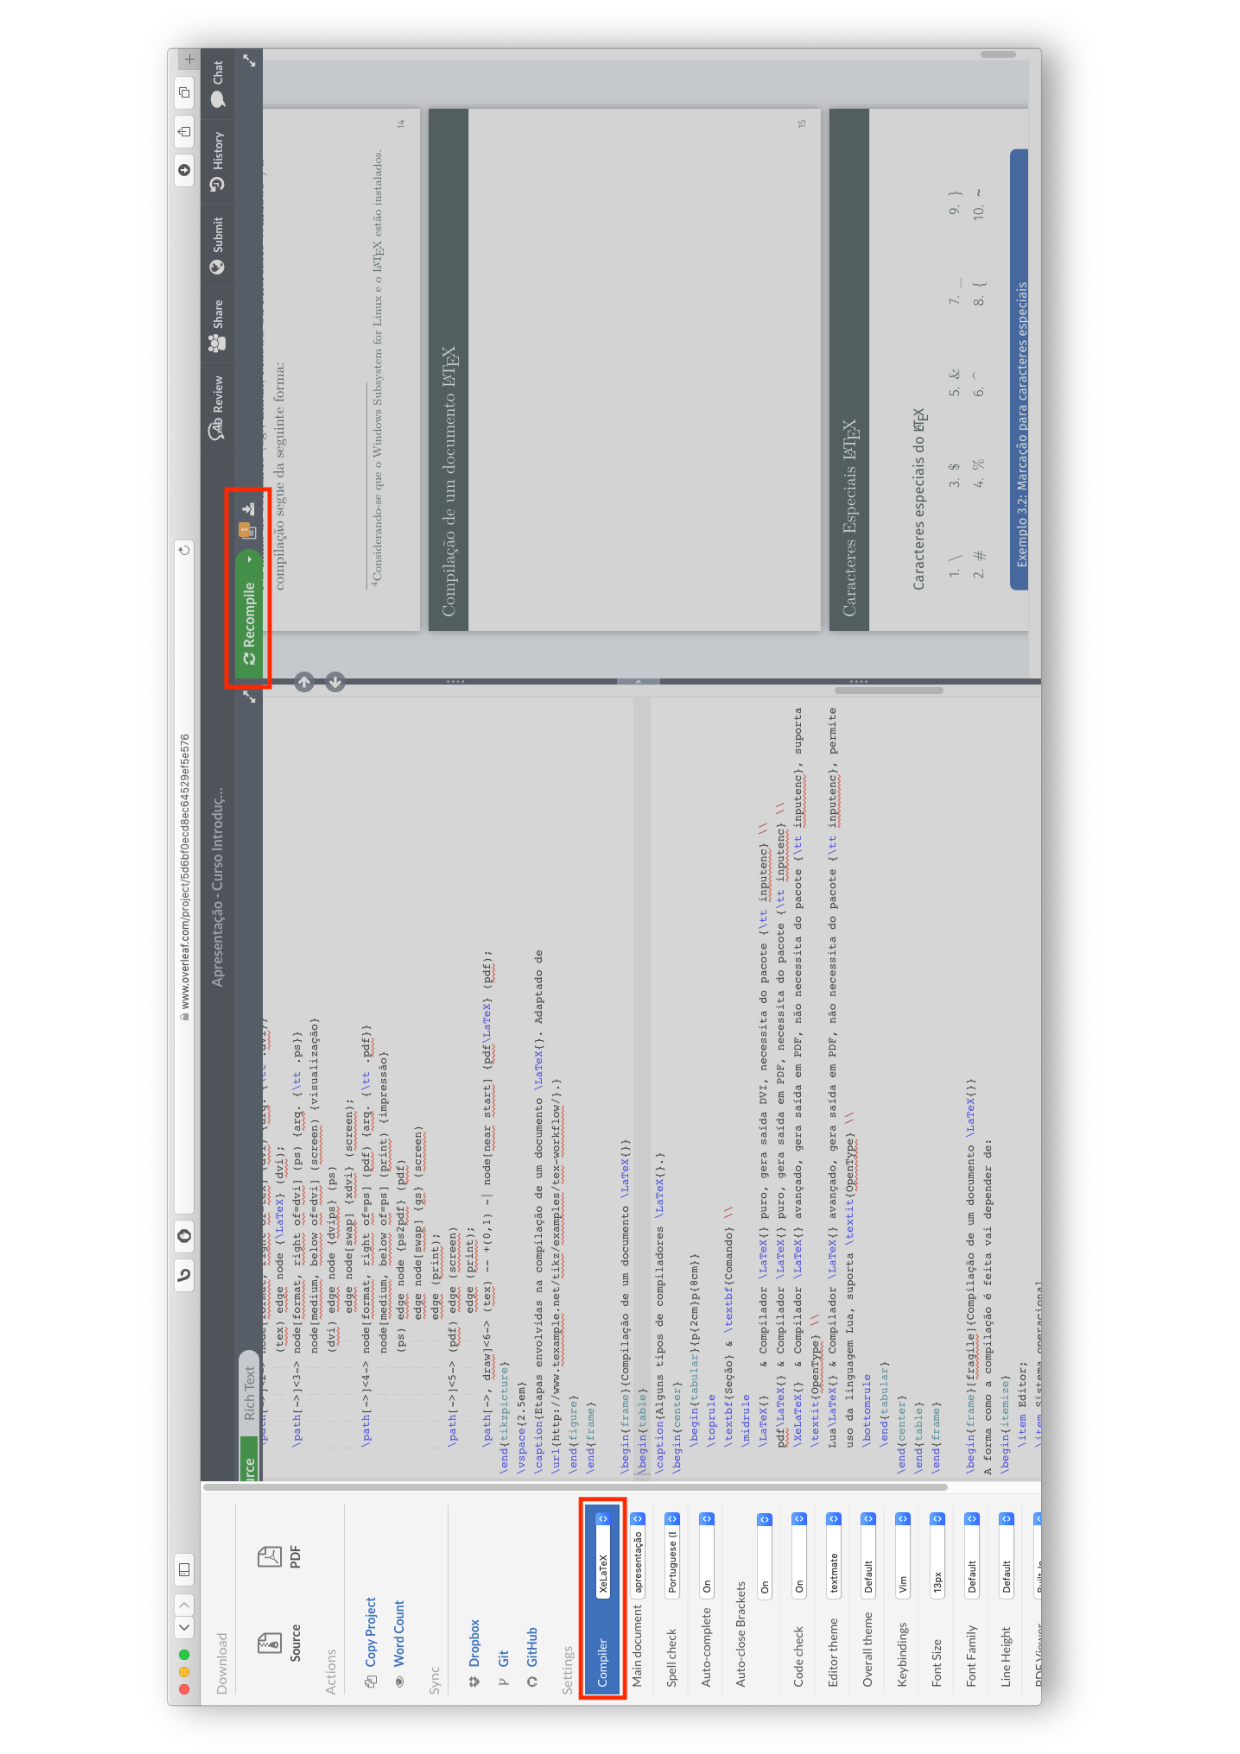
\includegraphics[width=0.65\textwidth,angle=-90]{./figs/overleaf.pdf}
		    \vspace{-2.5em}
		    \caption{Compilação de um documento \LaTeX{} no \textit{Overleaf} com o compilador \XeLaTeX{}.}
	    \end{figure}
    \end{block}
\end{frame}

\begin{frame}[fragile]{Localização e acentos}
    \begin{block}{Pacotes de idiomas}
        \begin{itemize}
            \item \mintinline{latex}{\usepackage[brazilian]{babel}}
            \item \mintinline{latex}{\usepackage[utf8]{inputenc}}\footnote{Não é necessário nos compiladores \XeLaTeX{} e Lua\LaTeX{}; já está pré-carregado nas versões mais recentes do \LaTeX{}.} ou
            \item \mintinline{latex}{\usepackage[latin1]{inputenc}}\footnote{Em desuso, utilize apenas se no seu computador os arquivos são salvos com a codificação ``ISO8859'', ``Western (Latin 1)'' ou ``Windows Latin 1''. }
        \end{itemize}
    \end{block}
    \begin{block}{Pacote de escrita (acentos e hifenização)}
        \begin{itemize}
            \item \mintinline{latex}{\usepackage[T1]{fontenc}}
        \end{itemize}
    \end{block}
\end{frame}

\subsection{Caracteres, símbolos especiais e acentos}

\begin{frame}[fragile]{Caracteres Especiais \LaTeX{}}
\begin{block}{Caracteres especiais do \LaTeX{}}
\begin{multicols}{5}
    \begin{enumerate}
        \item $\backslash$
        \item \#
        \item \$
        \item \%
        \item \&
        \item \^{}
        \item \_
        \item \{
        \item \}
        \item \texttt{\~{}}
    \end{enumerate}
\end{multicols}
\end{block}
    \begin{texexptitled}[center lower,enhanced,middle=2mm,listing side text]{Marcação para caracteres especiais}{exe_caracesp}
        $\backslash$
        \\  
        \^{}
        \\
        \texttt{\~{}}
    \end{texexptitled}
\end{frame}

\begin{frame}[fragile]{Localização e acentos}
\begin{texexptitled}[center lower,enhanced,middle=2mm,listing side text,righthand width=2.5cm]{Uso de acentos latinos no \LaTeX{}}{exe_acentos}
\'A \'E \'I \'O \'U

\'a \'e \'i \'o \'u

\^a \^A \~a \~A \`a \`A \~o \~O

\^e \^E \^o \^O

\"u \"U

\c{c} \c{C}
\end{texexptitled}
\end{frame}

\subsection{Tipos, tamanhos e estilos de letras}

\begin{frame}[fragile]{Tipos, tamanhos e estilos de letras}
\begin{texexptitled}[center lower, enhanced, middle=2mm, listing side text, righthand width=2cm]{Marcações mais mais comuns em fontes}{exe_estilos}
\textit{itálico}       \\
\textsl{inclinado}     \\
\underline{sublinhado} \\
\textbf{negrito}       \\
\textsuperscript{o}C   \\
H\textsubscript{2}O
\end{texexptitled}
\end{frame}

\begin{frame}[fragile]{Tipos, tamanhos e estilos de letras}
\begin{texexptitled}[center lower, enhanced, middle=2mm, listing side text, righthand width=2cm]{Tamanhos de fontes}{exe_tamfonte}
{\Huge Huge} \\
{\huge huge} \\
{\LARGE LARGE} \\
{\Large Large} \\
{\large large} \\
{\normalsize normalsize} \\
{\small small} \\
{\footnotesize footnotesize} \\
{\scriptsize scriptsize} \\
{\tiny tiny}
\end{texexptitled}
\end{frame}

\begin{frame}[fragile]{Tipos, tamanhos e estilos de letras}
\begin{texexptitled}[center lower,enhanced,middle=2mm]{Texto com diferentes tamanhos de fontes}{exe_tamfontefrase}
À noite, vovô {\large Kowalsky} vê o {\huge ímã} cair no {\small pé} do pinguim {\Huge queixoso} e vovó põe açúcar no {\footnotesize chá} de {\tiny tâmaras} do jabuti feliz. 
\end{texexptitled}
\end{frame}

\begin{frame}[fragile]{Tipos, tamanhos e estilos de letras}
\begin{texexptitled}[center lower,enhanced,middle=2mm]{Estilos de fontes, máquina de escrever ({\tt texttt})}{exe_font}
\texttt{Máquina de Escrever} | \texttt{\textit{Máquina de Escrever, em itálico}} | \texttt{\textsl{Máquina de Escrever, inclinado}}
\end{texexptitled}
\end{frame}

\begin{frame}[fragile]{Tipos, tamanhos e estilos de letras}
\begin{texexptitled}[center lower,enhanced,middle=2mm]{Estilos de fontes, sem serifa ({\tt textsf})}{exe_font}
\textsf{Sem Serifa} | \textsf{\textit{Sem Serifa, em itálico}} | \textsf{\textsl{Sem Serifa, inclinado}}
\end{texexptitled}
\end{frame}

\begin{frame}[fragile]{Tipos, tamanhos e estilos de letras}
\begin{texexptitled}[center lower,enhanced,middle=2mm]{Estilos de fontes, com serifa ({\tt textrm})}{exe_font}
\textrm{Com Serifa, estilo Romano} | \textrm{\textit{Com Serifa, estilo Romano itálico}} | \textrm{\textsl{Com Serifa, estilo Romano inclinado}}
\end{texexptitled}
\end{frame}

\subsection{Títulos e Seções}

\begin{frame}{Títulos e Seções}
\begin{table}
\caption{Títulos e Seções\footnote{Nem todas as classes possuem todas as seções. {\tt part} e {\tt chapter} funcionam apenas com as classes {\tt book} e {\tt report}.}}
\begin{center}
    \begin{tabular}{p{3cm}p{3cm}c}
    \toprule
    \textbf{Seção} & \textbf{Comando}                & \textbf{Nível} \\
    \midrule
    Parte          & \mintinline{latex}{\part}       & -1             \\
    Capítulo       & \mintinline{latex}{\chapter}    & 0              \\
    Seção          & \mintinline{latex}{\section}    & 1              \\
    Subseção       & \mintinline{latex}{\subsection} & 2              \\
    Parágrafo      & \mintinline{latex}{\par}        & 3              \\
    Subparágrafo   & \mintinline{latex}{\subpar}     & 4              \\
    \bottomrule
    \end{tabular}
\end{center}
\end{table}
\end{frame}

\subsection{Cores e Paletas de Cores}

\begin{frame}[fragile]{Cores e Paletas de Cores}
    \begin{block}{Paleta de cores padrão\footnote{Estas cores são fornecidas pelo pacote {\tt xcolor}.} do \LaTeX{}}
        \begin{center}
            \scalebox{0.7}{
                \begin{tikzpicture}
                    \fill [black] (0,0) rectangle ++(1.15,1.15);
                    \draw (0.615,-0.4) node {black};
                    \fill [blue] (1.75,0) rectangle ++(1.15,1.15);
                    \draw (2.365,-0.4) node {blue};
                    \fill [brown] (3.5,0) rectangle ++(1.15,1.15);
                    \draw (4.115,-0.4) node {brown};
                    \fill [cyan] (5.25,0) rectangle ++(1.15,1.15);
                    \draw (5.865,-0.4) node {cyan};
                    \fill [darkgray] (7,0) rectangle ++(1.15,1.15);
                    \draw (7.615,-0.4) node {darkgray};
                    \fill [gray] (8.75,0) rectangle ++(1.15,1.15);
                    \draw (9.365,-0.4) node {gray};
                    \fill [green] (10.5,0) rectangle ++(1.15,1.15);
                    \draw (11.115,-0.4) node {green};
                    \fill [lime] (12.25,0) rectangle ++(1.15,1.15);
                    \draw (12.865,-0.4) node {lime};
                    \fill [magenta] (14,0) rectangle ++(1.15,1.15);
                    \draw (14.615,-0.4) node {magenta};
                    
                    \fill [olive] (0,-1) rectangle ++(1.15,-1.15);
                    \draw (0.615,-2.65) node {olive};
                    \fill [orange] (1.75,-1) rectangle ++(1.15,-1.15);
                    \draw (2.365,-2.65) node {orange};
                    \fill [pink] (3.5,-1) rectangle ++(1.15,-1.15);
                    \draw (4.115,-2.65) node {pink};
                    \fill [purple] (5.25,-1) rectangle ++(1.15,-1.15);
                    \draw (5.865,-2.65) node {purple};
                    \fill [red] (7,-1) rectangle ++(1.15,-1.15);
                    \draw (7.615,-2.65) node {red};
                    \fill [teal] (8.75,-1) rectangle ++(1.15,-1.15);
                    \draw (9.365,-2.65) node {teal};
                    \fill [violet] (10.5,-1) rectangle ++(1.15,-1.15);
                    \draw (11.115,-2.65) node {violet};
                    \draw[fill=white] (12.25,-1) rectangle ++(1.15,-1.15);
                    \draw (12.865,-2.65) node {white};
                    \fill [yellow] (14,-1) rectangle ++(1.15,-1.15);
                    \draw (14.615,-2.65) node {yellow};
                \end{tikzpicture}
            }
        \end{center}
    \end{block}
\end{frame}

%\begin{frame}[fragile]{Cores e Paletas de Cores}
%\begin{texexptitled}[center lower,enhanced,middle=2mm]{Texto com fonte colorida, paleta padrão}{exe_cor1}
%\textit{\color{pink}{Quem} \color{cyan}{traz} \color{green}{CD}, \color{olive}{LP}, \color{violet}{fax}, \color{blue}{engov} \color{red}{e} \color{lime}{whisky} \color{orange}{JB?}}
%\end{texexptitled}
%\end{frame}

\begin{frame}[fragile]{Cores e Paletas de Cores}
\begin{texexptitled}[center lower,enhanced,middle=2mm]{Texto com fundo colorido, paleta padrão}{exe_cor3}
\textit{\colorbox{pink}{Quem} \colorbox{cyan}{traz} \colorbox{green}{CD}, \colorbox{olive}{LP}, \colorbox{violet}{\color{white}{fax}}, \colorbox{blue}{\color{white}{engov}} \colorbox{red}{e} \colorbox{lime}{whisky} \colorbox{orange}{JB?}}
\end{texexptitled}
\end{frame}

%\begin{frame}[fragile]{Cores e Paletas de Cores}
%    \begin{block}{Paleta de cores do projeto \textit{Solarized}\footnote{Estas cores são fornecidas pelo pacote {\tt xcolor-solarized}.} do \LaTeX{}}
%        \begin{center}
%            \scalebox{0.7}{
%                \begin{tikzpicture}
%                \fill [solarized-base03] (0,0) rectangle ++(1.15,1.15);
%                \draw (0.615,-0.4) node {base03};
%                \fill [solarized-base02] (1.75,0) rectangle ++(1.15,1.15);
%                \draw (2.365,-0.4) node {base02};
%                \fill [solarized-base01] (3.5,0) rectangle ++(1.15,1.15);
%                \draw (4.115,-0.4) node {base01};
%                \fill [solarized-base00] (5.25,0) rectangle ++(1.15,1.15);
%                \draw (5.865,-0.4) node {base00};
%                \fill [solarized-base0] (7,0) rectangle ++(1.15,1.15);
%                \draw (7.615,-0.4) node {base0};
%                \fill [solarized-base1] (8.75,0) rectangle ++(1.15,1.15);
%                \draw (9.365,-0.4) node {base1};
%                \fill [solarized-base2] (10.5,0) rectangle ++(1.15,1.15);
%                \draw (11.115,-0.4) node {base2};
%                \fill [solarized-base3] (12.25,0) rectangle ++(1.15,1.15);
%                \draw (12.865,-0.4) node {base3};
%                
%                \fill [solarized-yellow] (0,-1) rectangle ++(1.15,-1.15);
%                \draw (0.615,-2.65) node {yellow};
%                \fill [solarized-orange] (1.75,-1) rectangle ++(1.15,-1.15);
%                \draw (2.365,-2.65) node {orange};
%                \fill [solarized-red] (3.5,-1) rectangle ++(1.15,-1.15);
%                \draw (4.115,-2.65) node {red};
%                \fill [solarized-magenta] (5.25,-1) rectangle ++(1.15,-1.15);
%                \draw (5.865,-2.65) node {magenta};
%                \fill [solarized-violet] (7,-1) rectangle ++(1.15,-1.15);
%                \draw (7.615,-2.65) node {violet};
%                \fill [solarized-blue] (8.75,-1) rectangle ++(1.15,-1.15);
%                \draw (9.365,-2.65) node {blue};
%                \fill [solarized-cyan] (10.5,-1) rectangle ++(1.15,-1.15);
%                \draw (11.115,-2.65) node {cyan};
%                \fill [solarized-green] (12.25,-1) rectangle ++(1.15,-1.15);
%                \draw (12.865,-2.65) node {green};
%                \end{tikzpicture}
%            }
%        \end{center}
%    \end{block}
%\end{frame}

%\begin{frame}[fragile]{Cores e Paletas de Cores}
%\begin{texexptitled}[center lower,enhanced,middle=2mm]{Texto com fundo colorido, paleta \textit{Solarized}}{exe_corsol}
%\textit{\colorbox{solarized-magenta}{Quem} \colorbox{solarized-cyan}{traz} \colorbox{solarized-green}{CD}, \colorbox{solarized-red}{LP}, \colorbox{solarized-violet}{fax}, \colorbox{solarized-base1}{engov} \colorbox{solarized-red}{e} \colorbox{solarized-yellow}{whisky} \colorbox{solarized-orange}{JB?}}
%\end{texexptitled}
%\end{frame}
%
%\begin{frame}[fragile]{Cores e Paletas de Cores}
%    \begin{block}{Paleta de cores do projeto \textit{Material Design}\footnote{Estas cores são fornecidas pelo pacote {\tt xcolor-material}.} do Google}
%        \begin{center}
%            \scalebox{0.7}{
%                \begin{tikzpicture}
%                \fill [MaterialRed] (0,0) rectangle ++(1.15,1.15);
%                \draw (0.615,-0.4) node {red};
%                \fill [MaterialPink] (1.75,0) rectangle ++(1.15,1.15);
%                \draw (2.365,-0.4) node {pink};
%                \fill [MaterialPurple] (3.5,0) rectangle ++(1.15,1.15);
%                \draw (4.115,-0.4) node {purple};
%                \fill [MaterialDeepPurple] (5.25,0) rectangle ++(1.15,1.15);
%                \draw (5.865,-0.4) node {d. purple};
%                \fill [MaterialIndigo] (7,0) rectangle ++(1.15,1.15);
%                \draw (7.615,-0.4) node {indigo};
%                \fill [MaterialBlue] (8.75,0) rectangle ++(1.15,1.15);
%                \draw (9.365,-0.4) node {blue};
%                \fill [MaterialLightBlue] (10.5,0) rectangle ++(1.15,1.15);
%                \draw (11.115,-0.4) node {l. blue};
%                \fill [MaterialCyan] (12.25,0) rectangle ++(1.15,1.15);
%                \draw (12.865,-0.4) node {cyan};
%                \fill [MaterialTeal] (14,0) rectangle ++(1.15,1.15);
%                \draw (14.615,-0.4) node {teal};
%                
%                \fill [MaterialGreen] (0,-1) rectangle ++(1.15,-1.15);
%                \draw (0.615,-2.65) node {green};
%                \fill [MaterialLightGreen] (1.75,-1) rectangle ++(1.15,-1.15);
%                \draw (2.365,-2.65) node {l. green};
%                \fill [MaterialLime] (3.5,-1) rectangle ++(1.15,-1.15);
%                \draw (4.115,-2.65) node {lime};
%                \fill [MaterialYellow] (5.25,-1) rectangle ++(1.15,-1.15);
%                \draw (5.865,-2.65) node {yellow};
%                \fill [MaterialAmber] (7,-1) rectangle ++(1.15,-1.15);
%                \draw (7.615,-2.65) node {amber};
%                \fill [MaterialOrange] (8.75,-1) rectangle ++(1.15,-1.15);
%                \draw (9.365,-2.65) node {orange};
%                \fill [MaterialDeepOrange] (10.5,-1) rectangle ++(1.15,-1.15);
%                \draw (11.115,-2.65) node {d. orange};
%                \fill [MaterialBrown] (12.25,-1) rectangle ++(1.15,-1.15);
%                \draw (12.865,-2.65) node {brown};
%                \fill [MaterialGrey] (14,-1) rectangle ++(1.15,-1.15);
%                \draw (14.615,-2.65) node {grey};
%                \end{tikzpicture}
%            }
%        \end{center}
%    \end{block}
%\end{frame}
%
%\begin{frame}[fragile]{Cores e Paletas de Cores}
%\begin{texexptitled}[center lower,enhanced,middle=2mm]{Texto com fundo colorido, paleta \textit{Material Design}}{exe_cormaterial}
%\textit{\colorbox{MaterialRed}{Quem} \colorbox{MaterialPink}{traz} \colorbox{MaterialPurple}{CD}, \colorbox{MaterialDeepPurple}{LP}, \colorbox{MaterialIndigo}{\color{white}{fax}}, \colorbox{MaterialLightBlue}{\color{white}{engov}} \colorbox{MaterialTeal}{e} \colorbox{MaterialGreen}{whisky} \colorbox{MaterialLightGreen}{JB?}}
%\end{texexptitled}
%\end{frame}

\begin{frame}[fragile]{Cores e Paletas de Cores}
\begin{texexptitled}[center lower,enhanced,middle=2mm]{Definindo cores personalizadas}{exe_cor4}
\definecolor{meuazul1}{HTML}{0066ff}
\definecolor{meuazul2}{rgb}{0.2,0.6,1}
\definecolor{meuazul3}{RGB}{0,204,255}
\definecolor{meuazul4}{cmyk}{0.6,0,0,0}

\textit{Quem traz \colorbox{meuazul1}{\color{white}{CD}}, \colorbox{meuazul2}{\color{white}{LP}}, \colorbox{meuazul3}{\color{white}{fax}}, \colorbox{meuazul4}{\color{white}{engov}} e whisky JB?}
\end{texexptitled}
\end{frame}

\subsection{Medidas e Macros de Medidas}

\begin{frame}{Medidas}
\begin{table}
\centering
\caption{Unidades de Medidas mais Comuns no \LaTeX{}.}
    \begin{tabular}{p{3cm}cc}
    \toprule
    \textbf{Unidade} & \textbf{Abreviação} & \textbf{Valor em Pontos}              \\
    \midrule
    Ponto            & {\tt pt}.           & 1 {\tt pt}                            \\
    Milímetro        & {\tt mm}.           & 1 {\tt mm} = 2,84 {\tt pts}           \\
    Centímetro       & {\tt cm}.           & 1 {\tt cm} = 28,4 {\tt pts}           \\
    Polegada         & {\tt in}.           & 1 {\tt in} = 72,27 {\tt pts}          \\
    Paica             & {\tt pc}.           & 1 {\tt pc} = 12 {\tt pts}            \\
    Altura de ``x''  & {\tt ex}.           & \textit{Depende da fonte utilizada}   \\
    Altura de ``M''  & {\tt em}.           & \textit{Depende da fonte utilizada}   \\
    \bottomrule
    \end{tabular}
\end{table}
\end{frame}

\begin{frame}{Medidas}
\begin{table}
    \label{tab:medidas}
	\centering
	\caption{Algumas Macros de Medidas do \LaTeX{}.}
	\vspace{-1em}
	\begin{tabular}{p{3cm}p{7cm}}
		\toprule
		\textbf{Macro}                    & \textbf{Descrição}                                 \\
		\midrule
		\mintinline{latex}{\paperwidth}   & Largura de uma página                              \\
		\mintinline{latex}{\paperheight}  & Altura de uma página                               \\
		\mintinline{latex}{\textheight}   & Altura do texto na página                          \\
		\mintinline{latex}{\textwidth}    & Largura do texto na página                         \\
		\mintinline{latex}{\parindent}    & Indentação de um parágrafo                         \\
		\mintinline{latex}{\parskip}      & Espaçamento extra entre parágrafos                 \\
		\mintinline{latex}{\baselineskip} & Distância vertical entre as linhas em um parágrafo \\
		\mintinline{latex}{\columnsep}    & Distância entre colunas de texto                   \\
		\mintinline{latex}{\columnwidth}  & Largura de uma coluna de texto                     \\
		\mintinline{latex}{\linewidth}    & Largura de uma linha em um ambiente local          \\
		\bottomrule
	\end{tabular}
\end{table}
\end{frame}

\begingroup
\setbeamercolor{background canvas}{bg=InpeLaranja!90}
\begin{frame}[plain,fragile]{}
\begin{texexptitled}[center, width=0.99\paperwidth, height=0.99\paperheight, enhanced jigsaw, middle=2mm, listing side comment, righthand width=3.25cm, compilable listing, run latex, run dvips, run ps2pdf, pdf comment, comment style={raster columns=1}, freeze pdf]{Largura relativa com a \textit{macro} {\tt textwidth}}{exe_meds1}
\documentclass{article}
\usepackage[utf8]{inputenc}
\usepackage{lipsum}
\usepackage{graphicx}
\title{Título}
\author{Nome}
\date{\today}
\begin{document}
\maketitle
\section{Uma Seção}
\lipsum[2]
\includegraphics[width=1.0\textwidth]
{example-image-a}
\lipsum[3]
\includegraphics[width=0.5\textwidth]
{example-image-b}
\end{document}
\end{texexptitled}
\end{frame}
\endgroup

\begin{frame}{Medidas}
\vspace{0.75em}
\begin{table}
\centering
\caption{Algumas Macros de Espaçamento do \LaTeX{}.}
    \vspace{-1.5em}
    \begin{tabular}{p{2cm}p{8cm}}
    \toprule
    \textbf{Macro} & \textbf{Descrição} \\
    \midrule
    \mintinline{latex}{\hspace}    & Adiciona espaço horizontal (pode utilizar qualquer unidade da Tabela \ref{tab:medidas}, incluindo valores negativos)     \\
    \mintinline{latex}{\vspace}    & Adiciona espaço vertical (pode utilizar qualquer unidade da Tabela \ref{tab:medidas}, incluindo valores negativos)       \\
    \mintinline{latex}{\smallskip} & Equivalente a \mintinline{latex}{\vspace{smallskipamount}}, onde {\tt smallskipamount} é relativo ao estilo do documento \\
    \mintinline{latex}{\medskip}   & Equivalente a \mintinline{latex}{\vspace{medskipamount}}, onde {\tt medskipamount} é relativo ao estilo do documento     \\
    \mintinline{latex}{\bigskip}   & Equivalente a \mintinline{latex}{\vspace{bigskipamount}}, onde {\tt bigskipamount} é relativo ao estilo do documento     \\
    \bottomrule
    \end{tabular}
\end{table}
\end{frame}

\subsection{Parágrafos}

\begin{frame}[fragile]{Parágrafos}
\begin{texexptitled}[enhanced,middle=2mm]{Parágrafos sem quebra de linha}{exe_par1}
\lipsumsentence[1-4] 
\lipsumsentence[5-8]
\end{texexptitled}
\end{frame}

\begin{frame}[fragile]{Parágrafos}
\begin{texexptitled}[enhanced,middle=2mm]{Parágrafos com quebra de linha, separados por uma linha em branco}{exe_par2}
\lipsumsentence[1-4]

\lipsumsentence[5-8]
\end{texexptitled}
\end{frame}

\begin{frame}[fragile]{Parágrafos}
\begin{texexptitled}[enhanced,middle=2mm]{Parágrafos com quebra de linha, separados por duas barras invertidas (\mintinline{latex}{\\})}{exe_par3}
\lipsumsentence[1-4] \\
\lipsumsentence[5-8]
\end{texexptitled}
\end{frame}

\begin{frame}[fragile]{Parágrafos}
\begin{texexptitled}[enhanced,middle=2mm]{Parágrafos separados pelo comando {\tt newline}}{exe_par4}
\lipsumsentence[1-4]
\newline
\lipsumsentence[5-8]
\end{texexptitled}
\end{frame}

\begin{frame}[fragile]{Parágrafos}
\begin{texexptitled}[enhanced,middle=2mm]{Novo parágrafo iniciado pelo comando {\tt par}}{exe_par5}
\lipsumsentence[1-4] \par
\lipsumsentence[5-8]
\end{texexptitled}
\end{frame}

\begin{frame}[fragile]{Parágrafos}
\begin{texexptitled}[enhanced,middle=2mm]{Novo parágrafo iniciado pelo comando {\tt par}, com recuo especial}{exe_par6}
\setlength{\parindent}{3em}

\lipsumsentence[1-4] \par
\lipsumsentence[5-8]
\end{texexptitled}
\end{frame}

\begin{frame}[fragile,plain]{}
\begin{texexptitled}[enhanced,middle=2mm]{Novo parágrafo iniciado pelo comando {\tt par}, com recuo ({\tt parindent}) e espaçamento ({\tt parskip}) especiais}{exe_par7}
\setlength{\parindent}{3em}
\setlength{\parskip}{1em}

\lipsumsentence[1-4] \par
\lipsumsentence[5-8]
\end{texexptitled}
\end{frame}

%\begin{frame}[fragile,plain]{}
%\begin{texexptitled}[enhanced,middle=2mm]{Novo parágrafo iniciado pelo comando {\tt par}, com recuo ({\tt parindent}), espaçamento entre parágrafos ({\tt parskip}) e altura de linha ({\tt baselinestretch}) especiais}{exe_par8}
%\setlength{\parindent}{3em}
%\setlength{\parskip}{1em}
%\renewcommand{\baselinestretch}{1.6em}
%
%\lipsumsentence[1-3] \par
%\lipsumsentence[4-6]
%\end{texexptitled}
%\end{frame}

\begingroup
\setbeamercolor{background canvas}{bg=InpeLaranja!90}
\begin{frame}[plain,fragile]{}
\begin{texexptitled}[center,width=0.99\paperwidth,height=0.99\paperheight,enhanced jigsaw,middle=2mm,listing side comment,righthand width=4cm,compilable listing,run latex,run dvips,run ps2pdf,pdf comment,comment style={raster columns=1},freeze pdf]{Espaçamento de linha simples ({\tt baselinestretch, 1.0})}{exe_par8}
\documentclass{article}
\usepackage[utf8]{inputenc}
\usepackage{lipsum}

\renewcommand{
\baselinestretch}{1.0}

\begin{document}

\setlength{\parindent}{3em}
\setlength{\parskip}{1em}
\lipsum[1] \par
\lipsum[2]

\end{document}
\end{texexptitled}
\end{frame}
\endgroup

\begingroup
\setbeamercolor{background canvas}{bg=InpeLaranja!90}
\begin{frame}[plain,fragile]{}
\begin{texexptitled}[center,width=0.99\paperwidth,height=0.99\paperheight,enhanced jigsaw,middle=2mm,listing side comment,righthand width=4cm,compilable listing,run latex,run dvips,run ps2pdf,pdf comment,comment style={raster columns=1},freeze pdf]{Espaçamento de linha médio ({\tt baselinestretch, 1.3})}{exe_par9}
\documentclass{article}
\usepackage[utf8]{inputenc}
\usepackage{lipsum}

\renewcommand{
\baselinestretch}{1.3}

\begin{document}

\setlength{\parindent}{3em}
\setlength{\parskip}{1em}
\lipsum[1] \par
\lipsum[2]

\end{document}
\end{texexptitled}
\end{frame}
\endgroup

\begingroup
\setbeamercolor{background canvas}{bg=InpeLaranja!90}
\begin{frame}[plain,fragile]{}
\begin{texexptitled}[center,width=0.99\paperwidth,height=0.99\paperheight,enhanced jigsaw,middle=2mm,listing side comment,righthand width=4cm,compilable listing,run latex,run dvips,run ps2pdf,pdf comment,comment style={raster columns=1},freeze pdf]{Espaçamento de linha duplo ({\tt baselinestretch, 1.6})}{exe_par10}
\documentclass{article}
\usepackage[utf8]{inputenc}
\usepackage{lipsum}

\renewcommand{
\baselinestretch}{1.6}

\begin{document}

\setlength{\parindent}{3em}
\setlength{\parskip}{1em}
\lipsum[1] \par
\lipsum[2]

\end{document}
\end{texexptitled}
\end{frame}
\endgroup

\begin{frame}[fragile]{Parágrafos}
\begin{texexptitled}[enhanced,middle=2mm]{Parágrafos centralizados, utilizando o ambiente \mintinline{latex}{center}}{exe_par5}
\begin{center}
\lipsumsentence[9-10] \\ 
\lipsumsentence[11-12]
\end{center}
\end{texexptitled}
\end{frame}

%\begin{frame}[fragile]{Parágrafos}
%\begin{texexptitled}[enhanced,middle=2mm]{Parágrafos centralizados, utilizando o marcador {\tt centering}}{exe_par6}
%\centering
%\lipsumsentence[9-10] \\ 
%\lipsumsentence[11-12]
%\end{texexptitled}
%\end{frame}

\begin{frame}[fragile]{Parágrafos}
\begin{texexptitled}[enhanced,middle=2mm]{Parágrafos alinhados à esquerda, utilizando o ambiente {\tt flushleft}}{exe_par7}
\begin{flushleft}
\lipsumsentence[9-10] \\ 
\lipsumsentence[11-12]
\end{flushleft}
\end{texexptitled}
\end{frame}

\begin{frame}[fragile]{Parágrafos}
\begin{texexptitled}[enhanced,middle=2mm]{Parágrafos alinhados à direita, utilizando o ambiente {\tt flushright}}{exe_par8}
\begin{flushright}
\lipsumsentence[9-10] \\ 
\lipsumsentence[11-12]
\end{flushright}
\end{texexptitled}
\end{frame}

%\begin{frame}[fragile]{Parágrafos}
%\begin{texexptitled}[enhanced,middle=2mm]{Parágrafos justificado, utilizando o ambiente  {\tt justify}}{exe_just}
%\begin{justify}
%\lipsumsentence[9-10] \\ 
%\lipsumsentence[11-12]
%\end{justify}
%\end{texexptitled}
%\end{frame}

%\subsection{Posição e espaçamento}
%
%\begin{frame}[fragile]{Posição e espaçamento}
%\begin{texexptitled}[enhanced,middle=2mm]{Espaçamento vertical, utilizando o comando {\tt vspace}}{exe_par9}
%\lipsumsentence[32-33]
%\vspace{1cm}
%\lipsumsentence[34-35]
%\end{texexptitled}
%\end{frame}
%
%\begin{frame}[fragile]{Posição e espaçamento}
%\begin{texexptitled}[enhanced,middle=2mm]{Espaçamento horizontal, utilizando o comando {\tt hspace}}{exe_par10}
%\hspace{2cm}\lipsumsentence[36-37] \\ 
%\lipsumsentence[38-39]
%\end{texexptitled}
%\end{frame}

\subsection{Notas de rodapé}

\begin{frame}[fragile]{Notas de rodapé}
\begin{texexptitled}[enhanced,middle=2mm]{Nota de rodapé, utilizando o marcador {\tt footnote}}{exe_rodape1}
À noite, vovô Kowalsky\footnote{Esta é uma nota de rodapé.} vê o ímã cair no pé do pinguim queixoso e vovó põe açúcar no chá de tâmaras do jabuti feliz\footnote{Este é uma outra nota de rodapé.}.
\end{texexptitled}
\end{frame}

\begin{frame}[fragile]{Notas de rodapé}
\begingroup
\renewcommand*{\thefootnote}{\alph{footnote}}
\begin{texexptitled}[enhanced,middle=2mm]{Nota de rodapé, utilizando os marcadores {\tt footnotemark} e {\tt footnotetext}}{exe_rodape2}
À noite, vovô Kowalsky vê o ímã\footnotemark[1] cair no pé do pinguim queixoso\footnotemark[2] e vovó põe açúcar no chá de tâmaras do jabuti feliz.

\footnotetext[1]{Esta é uma nota de rodapé.}
\footnotetext[2]{Esta é uma outra nota de rodapé.}
\end{texexptitled}
\endgroup
\end{frame}

%\begin{frame}{Notas de Rodapé}
%\begin{table}
%\centering
%\caption{Alguns estilos de notas de rodapé.}
%\vspace{-0.5em}
%\label{tab:estilos_notas_rodape}
%    \begin{tabular}{p{2cm}p{6cm}}
%    \toprule
%    \textbf{Comando} & \textbf{Descrição} \\
%    \midrule
%    {\tt arabic} & Produz índices com algarismos arábicos (e.g., 1, 2, 3, ...) \\
%    {\tt roman} & Produz índices com algarismos romanos em caixa baixa (e.g., i, ii, iii, ...) \\
%    {\tt Roman} & Produz índices com algarismos romanos em caixa alta (e.g., I, II, III, ...) \\
%    {\tt alph}  & Produz índices alfabéticos em caixa baixa (e.g., a, b, c, ...) \\
%    {\tt Alph}  & Produz índices alfabéticos em caixa alta (e.g., A, B, C, ...) \\
%    {\tt fnsymbol} & Produz uma sequência de símbolos \\
%    \bottomrule
%    \end{tabular}
%\end{table}    
%\end{frame}
%
%\begin{frame}[fragile,plain]{}
%\begingroup
%\renewcommand*{\thempfootnote}{\Roman{mpfootnote}}
%\begin{texexptitled}[enhanced,middle=2mm]{Nota de rodapé com referência em algarismos romanos}{exe_rodape4}
%\renewcommand{\thefootnote}{\Roman{footnote}}
%
%À noite, vovô Kowalsky vê o ímã\footnote{Esta é uma nota de rodapé.} cair no pé do pinguim queixoso\footnote{Esta é mais uma nota de rodapé.} e vovó põe açúcar no chá de tâmaras do jabuti feliz.
%\end{texexptitled}
%\endgroup
%\end{frame}
%
%\begin{frame}[fragile,plain]{}
%\begingroup
%\renewcommand{\thempfootnote}{\arabic{mpfootnote}}
%\begin{texexptitled}[enhanced,middle=2mm]{Nota de rodapé com referência algarismos arábicos}{exe_rodape5}
%\renewcommand{\thefootnote}{\arabic{footnote}}
%
%À noite, vovô Kowalsky vê o ímã\footnotemark[1] cair no pé do pinguim queixoso\footnotemark[2] e vovó põe açúcar no chá de tâmaras do jabuti feliz.
%
%\footnotetext[1]{Esta é uma nota de rodapé.}
%\footnotetext[2]{Esta é uma outra nota de rodapé.}
%\end{texexptitled}
%\endgroup
%\end{frame}

\subsection{Listas}

\begin{frame}[fragile]{Listas}
\begin{texexptitled}[enhanced, listing side text, righthand width=4cm]{Lista não ordenada utilizando o ambiente \mintinline{latex}{itemize}}{exe_lista1}
\begin{itemize}
    \item Item 1
    \item Item 2
    \item Item 3
\end{itemize}
\end{texexptitled}
\end{frame}

%\begin{frame}[fragile,plain]{}
%\begin{texexptitled}[enhanced,middle=2mm]{Lista não ordenada aninhada utilizando o ambiente \mintinline{latex}{itemize}}{exe_lista2}
%\begin{itemize}
%    \item Item 1
%    \begin{itemize}
%        \item Item 1.1
%        \item Item 1.2
%    \end{itemize}
%    \item Item 2
%\end{itemize}
%\end{texexptitled}
%\end{frame}

\begin{frame}[fragile]{Listas}
\begin{texexptitled}[enhanced, listing side text, righthand width=4cm]{Lista não ordenada utilizando o ambiente \mintinline{latex}{itemize} com símbolos diferentes}{exe_lista_simb1}
    \begin{itemize}
        \item[\#]    Item 1
        \item[--]    Item 2
        \item[@]     Item 3
        \item[$\to$] Item 4
    \end{itemize}
\end{texexptitled}
\end{frame}

%\begin{frame}[fragile]{Listas}
%\begin{texexptitled}[enhanced,middle=2mm]{Lista não ordenada utilizando o ambiente \mintinline{latex}{itemize} com símbolos diferentes}{exe_lista_simb2}
%    \begin{itemize}[label=$\to$]
%        \item Item 1
%        \item Item 2
%        \item Item 3
%        \item Item 4
%    \end{itemize}
%\end{texexptitled}
%\end{frame}

\begin{frame}[fragile]{Listas}
\begingroup
%\renewcommand{\labelenumi}{\arabic{enumi}.}
\begin{texexptitled}[enhanced, listing side text, righthand width=4cm]{Lista ordenada utilizando o ambiente \mintinline{latex}{enumerate}}{exe_lista3}
\begin{enumerate}
    \item Item 1
    \item Item 2
    \item Item 3
\end{enumerate}
\end{texexptitled}
\endgroup
\end{frame}

%\begin{frame}[fragile,plain]{}
%\begingroup
%\renewcommand{\labelenumi}{\arabic{enumi}.}
%\renewcommand{\labelenumii}{(\alph{enumii})}
%\renewcommand{\labelenumiii}{\roman{enumiii}.}
%\renewcommand{\labelenumiv}{\Alph{enumiv}.}
%\begin{texexptitled}[enhanced,middle=2mm]{Lista ordenada aninhada utilizando o ambiente \mintinline{latex}{enumerate}}{exe_lista4}
%\begin{enumerate}
%    \item Item 1
%    \begin{enumerate}
%        \item Item 1a
%        \begin{enumerate}
%            \item Item 1a.i
%        \end{enumerate}
%    \end{enumerate}
%\end{enumerate}
%\end{texexptitled}
%\endgroup
%\end{frame}

\subsection{Figuras e Ambientes de Figuras}

%\begin{frame}[fragile]{Figuras e Ambientes de Figuras}
%\begin{texexptitled}[enhanced,middle=2mm]{Incluindo figura com o comando {\tt includegraphics}}{exe_fig1}
%\includegraphics[width=3cm]{example-image-a} 
%\end{texexptitled}
%\end{frame}

%\begingroup
%\setbeamercolor{background canvas}{bg=InpeLaranja!90}
\begin{frame}[fragile,plain]{}
\begin{texexptitled}[center, enhanced, middle=2mm]{Incorporando uma figura com o comando {\tt includegraphics} dentro do ambiente {\tt figure}}{exe_ambfig}
\begin{figure}[H]
    \caption{Uma figura dentro do ambiente {\tt figure}.}
    \includegraphics[width=3cm]{example-image-a}
\end{figure}
\end{texexptitled}
\end{frame}
%\endgroup

\begin{frame}[fragile]{Figuras e Ambientes de Figuras}
\begin{table}
\centering
\caption{Opções de posicionamento\footnote{Pode-se utilizar também os ambientes {\tt center}, {\tt flushleft} e {\tt flushright} para posicionar as figuras dentro do ambiente {\tt figure}.} relativo do ambiente {\tt figure}.}
\vspace{-1em}
\label{tab:ambfig}
    \begin{tabular}{p{2cm}p{8cm}}
    \toprule
    \textbf{Opção} & \textbf{Descrição} \\
    \midrule
    {\tt h} & `aqui'' (\textit{here}). Posição exata pode variar de acordo com outros elementos \\
    {\tt t} & ``topo'' da página (\textit{top}) \\
    {\tt b} & ``base'' da página (\textit{bottom}) \\
    {\tt p} & ``página'' separada (\textit{page}) \\
    {\tt !} & Força a posição onde o ambiente se encontra (e.g., {\tt h!}) \\
    {\tt H} & Precisamente no local (depende do pacote {\tt float}; equivalente a {\tt h!}) \\
    \bottomrule
    \end{tabular}
\end{table}
\end{frame}

%\begin{frame}[fragile,plain]{}
%\begin{texexptitled}[enhanced,middle=2mm]{Citando uma figura}{exe_ambfig}
%\begin{figure}[H]
%    \label{fig:exe_img_a}
%    \caption{Uma figura.}
%    \includegraphics[width=2cm]{example-image-a}
%\end{figure}
%Outro texto digitado após a Figura \ref{fig:exe_img_a}
%\end{texexptitled}
%\end{frame}

%\begin{frame}[fragile,plain]{}
%\begin{texexptitled}[enhanced,middle=2mm]{Inserindo uma ou mais figuras lado-a-lado com o comando {\tt subfigure}}{exe:subfigure1}
%\begin{figure}[H]
%    \begin{center}
%        \subfigure[Figura ``A'']
%        {\includegraphics[width=0.25\textwidth]{example-image-a}}
%        \subfigure[Figura ``B'']
%        {\includegraphics[width=0.25\textwidth]{example-image-b}}
%    \end{center}
%\end{figure}
%\end{texexptitled}
%\end{frame}

%\begin{frame}[fragile,plain]{}
%\begin{texexptitled}[enhanced,middle=2mm]{Inserindo uma ou mais figuras lado-a-lado com o comando {\tt subfigure}}{exe:subfigure1}
%\begin{figure}[H]
%    \centering
%        \begin{subfigure}[b]{0.3\textwidth}
%            \includegraphics[width=0.25\textwidth]{example-image-a}
%            \caption{}
%            \label{}
%        \end{subfigure}
%        \begin{subfigure}[b]{0.3\textwidth}
%            \includegraphics[width=0.25\textwidth]{example-image-b}
%            \caption{}
%            \label{}
%    \end{subfigure}
%\end{figure}
%\end{texexptitled}
%\end{frame}

\subsection{Matemática e ambientes de equações}

\begin{frame}[fragile]{Matemática e ambientes de equações}
\begin{texexptitled}[center lower,enhanced,middle=2mm]{Inserindo equações em linha (\textit{inline})}{exe_eq0}
Uma equação do segundo grau tem a forma geral, $ax^2 + bx + c =0$. Suas raízes são calculadas por, $x = \frac{-b \pm \sqrt{b^2 - 4ac}}{2a}$.
\end{texexptitled}
\end{frame}

\begin{frame}[fragile,plain]{}
\begin{texexptitled}[center lower,enhanced,middle=2mm]{Ambientes {\tt equation} e {\tt equation*}}{exe_eq1}
\begin{equation*}
x = \frac{-b \pm \sqrt{b^{2} - 4ac}}{2a}
\end{equation*}

\begin{equation}
\label{eq1}
x = \frac{-b \pm \sqrt{b^{2} - 4ac}}{2a}
\end{equation}
\end{texexptitled}
\end{frame}

\begin{frame}[fragile]{Matemática e ambientes de equações}
\begin{texexptitled}[center lower,enhanced,middle=2mm]{Ambientes {\tt equation} e {\tt split}}{exe_eq2}
\begin{equation*}
\begin{split}
f(x) & = x^{-\frac{1}{2}}   \\
     & = \frac{1}{\sqrt{x}}\text{, }\forall x \neq 0.
\end{split}
\end{equation*}
\end{texexptitled}
\end{frame}

\begin{frame}[fragile,plain]{}
\begin{texexptitled}[center,enhanced,middle=2mm,width=0.92\paperwidth]{Ambiente {\tt multline}}{exe_eq3}
\begin{multline*}
A(x,y)\frac{\partial^2{\Psi}}{\partial{x^2}} + B(x,y)\frac{\partial^2{\Psi}}{\partial{x}\partial{y}} + C(x,y)\frac{\partial^2{\Psi}}{\partial{y^2}} + D(x,y)\frac{\partial{\Psi}}{\partial{x}} + \\ + E(x,y)\frac{\partial{\Psi}}{\partial{y}} + F(x,y)\Psi = G(x,y)
\end{multline*}
\end{texexptitled}
\end{frame}

\begin{frame}[fragile]{Matemática e ambientes de equações}
\begin{texexptitled}[center lower,enhanced,middle=2mm]{Ambiente {\tt align}}{exe_eq4}
\begin{align*}
e^{i\pi} + 1 & = 0 \\ 
           e & = \lim_{n \to \infty}{\Bigg(1 + \frac{1}{n}\Bigg)^{n}}  
\end{align*}
\end{texexptitled}
\end{frame}

\begin{frame}[fragile]{Matemática e ambientes de equações}
\begin{texexptitled}[center lower,enhanced,middle=2mm]{Ambiente {\tt gather}}{exe_eq5}
\begin{gather*}
 x           = 1 + 2y + 3z \\ 
3x -  y + 2z = 0           \\
2x +  y      = 2 - z
\end{gather*}
\end{texexptitled}
\end{frame}

\subsection{Tabelas}

\begin{frame}[fragile]{Tabelas}
\begin{texexptitled}[center, width=0.9\paperwidth, enhanced, listing side text, righthand width=3cm, middle=2mm]{Exemplo de uma tabela simples com o ambiente {\tt tabular}}{exe_tab1}
\begin{tabular}{c c}
\toprule
\textbf{L0C1} & \textbf{L0C2} \\
\midrule
L1C1 & L1C2 \\
L2C1 & L2C2 \\
L3C1 & L3C2 \\
\bottomrule
\end{tabular}
\end{texexptitled}
\end{frame}

%\begingroup
%\setbeamercolor{background canvas}{bg=InpeLaranja!90}
\begin{frame}[fragile,plain]{}
\begin{texexptitled}[center, enhanced, middle=2mm]{Exemplo de uma tabela simples com o ambiente {\tt tabular} e colunas mais largas}{exe_tab3}
\begin{tabular}{p{3cm}  p{5cm}}
\toprule 
\textbf{L0C1} & \textbf{L0C2} \\
\midrule
L1C1 & L1C2 \\
L2C1 & L2C2 \\
L3C1 & L3C2 \\
\bottomrule
\end{tabular}
\end{texexptitled}
\end{frame}

\begin{frame}[fragile,plain]{}
\begin{texexptitled}[center, enhanced, middle=2mm]{Exemplo de uma tabela simples utilizando o ambiente {\tt tabularx}}{exe_tab7}
\begin{tabularx}{\textwidth}{X | X | X}
\toprule
L0C1 & L0C2 & L0C3 \\
\midrule
L1C1 L1C1 & L1C2 L1C2 L1C2 L1C2 L1C2 L1C2 & L1C3 \\
L2C1 L2C1 & L2C2 L2C2 L2C2 L2C2 & L2C3 L2C3 \\
\bottomrule
\end{tabularx}
\end{texexptitled}
\end{frame}
%\endgroup

\end{document}
